\section{Tools}
\label{section:bcoollengbench}

\todo{Pictures: timing output, state space}

\begin{itemize}
	\item \bcool is a set of plugins for Eclipse Modeling Framework (EMF)\footnote{http://www.eclipse.org}. Its abstract syntax has been developed using Ecore (\ie the meta-language associated with EMF). The textual concrete syntax has been developed by using Xtext thus providing advanced editing facilities.
	
	\item \bcool is integrated into the GEMOC Studio, an Eclipse package atop EMF, which includes both a language workbench to design and implement tool-supported xDSMLs, and a modeling workbench where the xDSMLs are automatically deployed to allow system designers to edit, execute, simulate, and animate their models. \bcool takes advantages of this collaborative environment by adding coordination facilities. 
	
	\item In the language workbench, an integrator can develop operators by relying on the deployed languages. Language behavioral interfaces are automatically deployed and can be imported by a \bcool specification. To build its own libraries, the workbench provides \moccml thus helping the integrator to specify EventRelations and EventExpression.   
	
	\item Operators are automatically deployed into the modeling workbench and can be used by a system designer to generate a model of coordination. This task is automated by relying on a set of plugins. The workbench provides several tools to perform verification activities \eg execution and animation, space-state exploration, etc.  

	\item We implement the running example by using the GEMOC studio. We rely on the languages TFSM and Activity that can be automatically created by a wizard. Once deployed into the language workbench, we use \bcool to specify the operator in Listing~\ref{lst:bcoolrunningexample}. 
	
	\item In the model workbench, we use the deployed languages to build the models of the coffee machine. This corresponds with a TFSM and an Activity (see Figure~\ref{?}). Then, we use the workbench to execute and animate the models. Figure~\ref{?} illustrates the partial timing output of the execution of the whole example. The workbench also offers the possibility to obtain by exploration quantitative results on the scheduling state-space.    
	
	\item \todo{To talk about the resulting state space}

	\item \todo{A video showing the full workflow and the animation can be found in ?. To talk about the site}
\end{itemize}
  

\begin{figure}
	\begin{center}
		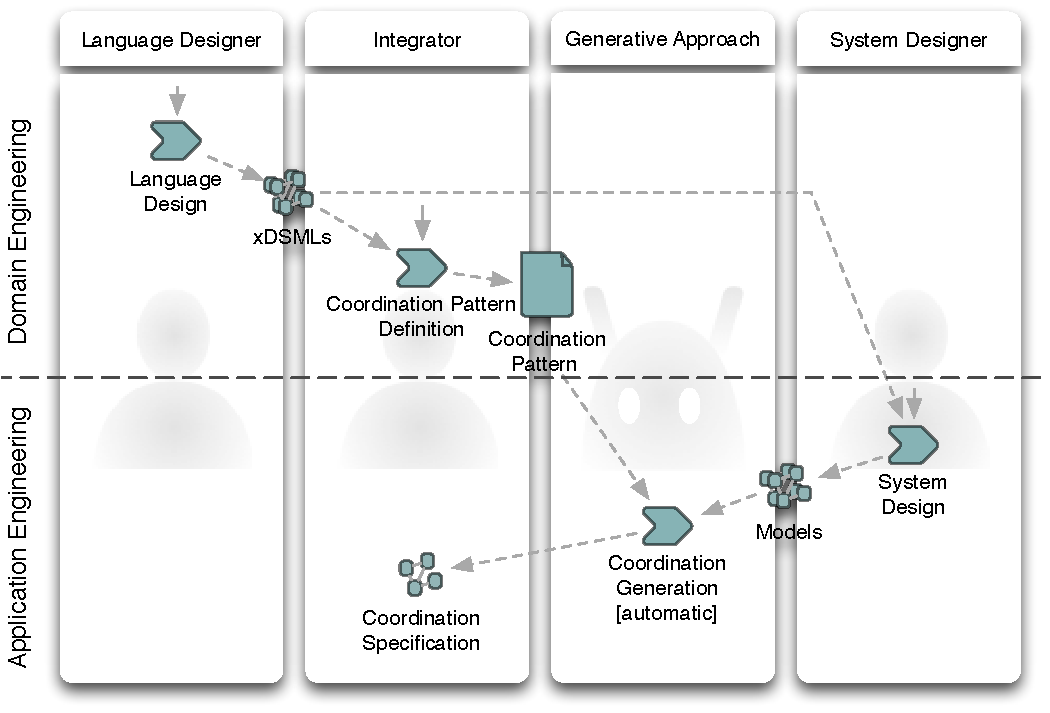
\includegraphics[width=.6\textwidth]{bcool/figs/process}
		\caption{The Proposed Workflow}
		\label{fig:proposedworkflow}
	\end{center}
\end{figure}

